\documentclass[12pt]{article}
%\documentclass[8pt,twocolumn]{article}

\usepackage[letterpaper, margin=0.75in]{geometry}
\usepackage{graphicx}
\usepackage{comment}
\usepackage{float}
\usepackage{hyperref}
\usepackage[authoryear]{natbib}
\usepackage{setspace}
\usepackage{mathtools}
%\usepackage{aas_macros}
\usepackage{amssymb}
\usepackage{textcomp}
\usepackage{siunitx}

%\onehalfspacing
\doublespacing

\title{The Aerosol Limb Imager: Acousto-Optic Measurements of Limb Scattered Sunlight for 2D Stratospheric Aerosol Profiles}

\author{Brenden J Elash, Adam E Bourassa, Paul R P Loewen, Douglas A Degenstein}

\begin{document}
\renewcommand\bibname{BiBTex.bib}

\maketitle

\abstract{The Aerosol Limb Imager (ALI) is a prototype atmospheric instrument developed at the University of Saskatchewan with the long term goal of a satellite mission to gather high resolution horizontal and vertical stratospheric aerosol profiles, including extinction and particle size. The immediate goal of the ALI prototype is to test and verify the use of an Acousto-Optical Tunable Filter (AOTF), the fundamental technology behind ALI, in a space environment and to gather atmospheric sulfate aerosol profiles with high spatial resolution. ALI will measure light from the atmosphere through the limb geometry which measures the radiance from scattered sunlight from sunlit atmosphere. ALI is a single channel instrument measuring radiance from the visible to the near infrared wavelengths (650-950~nm) and through successive images builds spectral information. The system uses a telescopic front end to pass collimated light through the AOTF for each line of sight which is then focused onto the the detector. The AOTF has the property of separating the incoming radiance into each of its linear polarized components and rotating the selected wavelength's polarization by 90\si{\degree} allowing one to recover some polarization information of the incoming radiance. The ALI prototype was completed in August of 2014. A stratospheric balloon test flight from the Canadian Space Agency (CSA) balloon launch facility in Timmins, Ontario onboard the CNES CARMEN-2 gondola platform occurred on September 20, 2014. The data from the flight undergoes a method to convert the data into relative radiances and are used in a MART retrieval method to determine aerosol extinction and size profiles.}

\section{Introduction}
\label{sec:introduction}

Aerosol has been monitored in several different geometries throughout history. Occultation was one of the first methods used on satellite instrumentation to measure atmospheric species, including ozone. Notable instruments included SAM II \citep{McCormick1979}, SAGE II \citep{McCormick1987}, and SAGE III \citep{Thomason2003}. Another geometry is the limb scatter geometry which measures radiance from the sunlit atmosphere as it scatters and interacts with molecules. However, the limb scatter geometry has a complexity that requires a forward model to be able to accurately compute the scattering interactions, both single and multiple, between different constituents. Limb scatter was first preformed on the Solar Mesosphere Explorer (SME) \citep{Barth1983} to measure ozone profiles in 1981. Two instruments from the previous generation of remote sensing instruments have successfully used limb scatter to determine aerosol atmospheric parameters, the Optical Spectrograph and InfraRed Imaging System (OSIRIS) a Canadian instrument onboard the Odin satellite \citep{Llewellyn2004} and SCanning Imaging Absorption spectroMeter for Atmospheric CHartographY (SCIAMACHY) onboard the ENVISAT \citep{Bovensmann1999} which are grating spectrometers that acquire data at a single altitude at a time so a series of exposures is required to create a vertical profile with approximately a 1.5~km and 3~km vertical resolution for OSIRIS and SCIAMACHY respectively. The Ozone Mapping Profiler Suite - Limb Profiler (OMPS-LP) \citep{Rault2013} is a current generation instrument which images the atmosphere with spectral and vertical spatial information with 1~km vertical resolution and measures ozone and aerosol parameters. The proposed method with ALI allows for two dimensional spatial images of a wavelength with polarized light scanned spectrally giving both vertical and horizontal resolution of the environment through the use of the innovative AOTF technology. Aerosol is a broadband scattering feature with effects that can been observed from a wide range of wavelengths from 525~nm extending into the near infrared and does not require high spectral resolution in order to determine aerosol extinction profiles.

%Different instrumentation techniques were also put into space to acquire atmospheric data for different species with differing resolutions and quantity of data that could be acquired in a single day.

Sulfuric aerosol is a fundamental portion of the global climate balance. Stratospheric aerosol loading has been increasing at a rate of 4-7\% per year from 2002 to 2009 due to moderate volcanic eruptions \citep{Vernier2011} which have lead to a negative radiative forcing effect that has partially offset the radiative forcing from CO$_{2}$ \citep{Solomon2011}. Aerosol is a spherical partical that scatters incoming radiance away from the surface of the planet causing an overall cooling effect which is dependant on extinction and particle size distribution \citep{Kiehl1993}. This effect is fully defined by aerosol microphysics requiring accurate knowledge of concentration and particle size distributions. The method of aerosol transportation across the tropopause are not completely understood, recently, after the 2011 eruption of Nabro it was determined that the asian monsoon has the ability to penetrate through the thermal boundary and ejected aerosol from the Nabro plume into the stratosphere \citep{Bourassa2012c}. Also anthropogenic sources of SO$_{2}$ can enter the stratosphere  through the Asian tropopause aerosol layer that forms during the Asian monsoon \citep{Vernier2011, Neely2014}.

A lidar instrument, CALIPSO, is able to achieve aerosol profiles of 333~m horizontal resolution and 60~m, 180~m, and 300~m vertical resolution for the altitude ranges of 8.2-20.2~km, 20.2-30.1~km, and 30.1-40.0~km respectively \citep{Winker2003}. Additional instrumentation with high resolutions on the order of 150~m vertically and horizontally will satisfy the needs for current scientific investigation and will allow the determination of aerosol loading from volcanic and anthropogenic sources causing a surface cooling effect and as well account for losses from the stratosphere due to transportation that will counteract the previous cooling effect. ALI, a prototype for a next generation of instruments will address the much needed horizontal and vertical resolution previously stated required to help answer questions about global climate. The ALI prototype discussed in the work has been designed with balloon geometries in mind, accounting for a larger field of view to be able to image the whole limb with a range of 35~km vertically and horizontally as well. However, for satellite geometry with a low earth orbit (approximately 600~km) a considerable smaller field of view will be required to have the same 35x35km field of view.

%Work by \cite{Andreae2005} has shown that global warming has not been as drastic as perviously expected due to the high amounts of aerosol in the stratosphere currently due to the high volcanic activity.

%Furthermore, high resolution aerosol measurements are required in order to be able to determine aerosol extinction ratios during high aerosol loading due to the long path length and high amounts of scattering.

In this paper, the first section will outline the technology behind the AOTF used within the ALI system. Following is a description of the optical design behind ALI including an ulterior optical presentation comparing the benefits and drawbacks between two optical layout which will be followed by a comparison with the Belgium instrument ALTIUS \citep{Dekemper2012}. An overview of ALI's maiden flight, including the conditions and trajectory of the flight, onboard the CNES CARMEN-2 gondola from the CSA balloon launch facility in Timmins, Ontario will be presented. Post flight analysis of the data is presented including the measurements taken during the campaign, the conversion from raw measurements into calibrated data, and an retrieval algorithm for aerosol extinction and particle size parameters will be outlined and then preformed on the data from the campaign.

\section{Instrument Design}

\subsection{Acouto-Optical Tunable Filter Characteristics}

%where $\mathbf{k}_{i}$ and $\mathbf{k}_{d}$ are the wave vectors for the incoming and diffracted light and $\boldsymbol\kappa$ is the acoustic wave vector. These wave vectors can be described by
%\begin{equation}
%    \ k_{i} = \frac{2\pi n_{i}}{\lambda}
%    \label{eqn:3.1:incomingWavevector}
%\end{equation}
%\begin{equation}
%    \ k_{d} = \frac{2\pi n_{d}}{\lambda}
%    \label{eqn:3.1:diffractedWavevector}
%\end{equation}
%\begin{equation}
%    \ \kappa = \frac{2\pi F}{\nu}
%    \label{eqn:3.1:acousticWavevector}
%\end{equation}
%where $n_{i}$ and $n_{d}$ are the indices of refraction of incoming and diffracted light. Finally $\lambda$ is the wavelength of light in a vacuum. It will be assumed that the extraordinary light is undergoes the momentum matching through the device. This causes the above refractive indices defined above to be
%\begin{equation}
%    \ n_{i} = \left( \frac{\sin^{2}(\theta_{i}+\alpha)}{n_{e}^{2}} + \frac{\cos^{2}(\theta_{i}+\alpha)}{n_{o}^{2}} \right)^{-\frac{1}{2}}
%    \label{eqn:3.1:incomingIndexOfRefraction}
%\end{equation}
%\begin{equation}
%    \ n_{d} = n_{o}
%    \label{eqn:3.1:diffractedIndexOfRefraction}
%\end{equation}
%where $n_{e}$ and $n_{o}$ are the indices of refraction for the extraordinary and ordinary polarizations of the incoming light and $\alpha$ is the cut angle relative to the piezoelectric transducer and the optical axis. For a crystal, like TeO$_{2}$, the difference in the index of refraction is small and can be approximated as \citep{Voloshinov2007}
% \begin{equation}
%    \ n_{i} = n_{o} + \Delta n\sin^{2}(\theta_{i}+\alpha)
%    \label{eqn:3.1:incomingIndexOfRefractionApprox}
%\end{equation}
%where $\Delta n$ is the difference between the extraordinary and ordinary indices of refraction (ie $\Delta n = n_{e} - n_{o}$). The wave vectors, seen in \autoref{fig:3.1:ATOFWavevectors}, of the system need to follow the momentum matching criteria from \autoref{eqn:3.1:phaseMatching}. Separating the wave vectors into their directional components with respect to the cut angle, $\alpha$, the tangential and perpendicular directions respectively are
%\begin{equation}
%    \ k_{i}\cos\theta_{i} = {k}_{d}\cos\theta_{d}
%    \label{eqn:3.1:wavevectorsTangentalDirection}
%\end{equation}
%\begin{equation}
%    \ k_{i}\sin\theta_{i} + \kappa = {k}_{d}\sin\theta_{d}
%    \label{eqn:3.1:wavevectorsPerepndicularDirection}
%\end{equation}

An AOTF uses an acoustic wave, set by a Radio Frequency (RF), that is prorogated through the crystal and forms a standing wave to allow the diffraction of a specific wavelength causing a filtering effect. The use of an AOTF for an imaging system has several distinct advantages due to its low mass, fast stabilization times of a few microseconds, no moving parts, and has only recently become possible thanks to improvements to non-collinear acosto devices with the use of birefringent materials with large apertures \citep{Chang1974, Voloshinov2007} which allowed for the ability to image with AOTF technology. In order for the AOTF to allow the diffraction of a specific wavelength a momentum matching criteria must be held where the wave vectors of the acoustic wave match the difference of the incoming and diffracted light wave vectors as seen in \autoref{fig:3.1:ATOFWavevectors}. This condition is known as the Bragg matching criteria and is given by
\begin{equation}
    \ \mathbf{k}_{i} = \boldsymbol\kappa + \mathbf{k}_{d}
    \label{eqn:3.1:phaseMatching}
\end{equation}
where $\left|\mathbf{k}_{i}\right| = \frac{2\pi n_{i}}{\lambda}$ is the momentum of the incoming light, $\left|\mathbf{k}_{d}\right| = \frac{2\pi n_{d}}{\lambda}$ is the momentum of the diffracted light, and $\left|\boldsymbol\kappa\right| = \frac{2\pi F}{\nu}$ is the momentum of the acousto wave. The parameters $\lambda$, $F$, and $\nu$ are the wavelength in vacuum, the frequency of the RF wave, and the phase velocity in the crystal respectively. Using the condition given in \autoref{eqn:3.1:phaseMatching} and the wave vector diagram gives the following relation for a birefringent material undergoing Bragg diffraction
\begin{equation}
    \lambda  = \frac{\Delta n\nu}{F}\frac{\sin^{2}(\theta_{i}+\alpha)}{\sin\theta_{i}}
    \label{eqn:3.1:AOTFWavelengthDependance}
\end{equation}
where $\Delta n$ is the absolute difference between the ordinary and extraordinary indices of refraction, $\theta_{i}$ is the angle of incidence of the incoming light, and $\alpha$ is the cut angle which is the angle from the optical axis to the piezoelectric transducer. Also, through the described interaction the diffracted light goes though a 90\si{\degree} rotation in polarization \citep{Voloshinov1996}.

In order to be able to preform the required spectral imaging a 10x10~mm aperture imaging quality ATOF was acquired from Brimrose of America. It is optically tuned, meaning designed for a specific wavelength octave, for a range of 600 to 1200~ nm corresponding to a RF range of 156 to 70~MHz and made from Tellurium Dioxide (TeO$_{2}$), a birefringent crystal with indices of refraction at 800~nm of 2.226 and 2.373 for the ordinary and extraordinary modes respectively \citep{Uchida1971}. The extraordinary light is diffracted at 2.7 degrees off of the optical axis of the device. In order to achieve a constant diffraction angle of the first order beam a wedge is attached to the exit aperture of the AOTF to compensate for the angular change that occurs from altering the wavelength. The ordinary light undergoes diffraction but at a nonconstant angle off of the optical axis with respect to wavelength due to the ordinary polarization being uncompensated. It is important to note that it is currently not possible to have both polarizations compensated and as such only one polarization will be captured by ALI.

Characterization of the AOTF is required for calibrated use in an instrument. For characterization, the AOTF is surrounded by a telocentric front and back end since it will allow the best determination of the central wavelength of the device at a sacrifice of the optimal FWHM results. Also linear polarizers were inserted before and after the AOTF to remove undesired signals. A 100~mm plano-convex lenses were chosen for both lenses to best fill the AOTF aperture. The light source is a 100~W quartz-tungsten halogen bulb that is collimated and passed into the first telocentric lens. The light passes though the AOTF focused then is re-collimated through the second lens. The signal enters a HORIBA iHR320 spectrometer with a minimum spectral resolution of 1.175~nm. The spectral results were imaged on a Synapse 354308 front-illuminated CCD detector with 1024x256 pixels. Images were taken at a set of RFs spaced every 150~kHz from 75~MHz to 160~MHz. For each image the results are spectrally averaged across the rows and a typical spectral measurement result can be seen in the panel (a) of \autoref{fig:3.1:AOTFCharaterization}. The maximum value of each image is taken to be the central wavelength through the AOTF at each respective RF.

The maximum values from each of the images were determined as well as the corresponding wavelengths for these values. It was noted that the curve appears to follow a power function of the form
\begin{equation}
    \ F = a\lambda^{b}.
    \label{eqn:3.1:powerFunction}
\end{equation}
A linear least squares fit was preformed in log space finding the coefficients $a$ and $b$. The fit was performed and appeared to match the data quite well but a relative error analysis was preformed and it was seen that there was a only an agreement better than 0.6\% within the testing range and would increase for wavelengths outside the testing region. A better fit was desired to characterize the AOTF's RF-spectral dependance so a modified power function was used in the form of
 \begin{equation}
    \ F = a\lambda^{b+c\log\lambda}
    \label{eqn:3.1:modifiedPowerFunction}
\end{equation}
or a quadratic least squares fit. These results can be seen in panels (c) and (d) of \autoref{fig:3.1:AOTFCharaterization}. The agreement of this form is less than 0.1\% throughout the whole wavelength range and the determined RF and wavelength relation can be seen in
\begin{equation}
    \ F = \exp{(19.793)}\lambda^{-3.381+0.168\log\lambda}
    \label{eqn:3.1:modifiedPowerFunctionCoeffiecicents}
\end{equation}
where $\lambda$ is in nanometers and $F$ is in MHz. It should be noted that even though the AOTF optical range is 600~nm to 1200~nm this analysis only measures wavelengths from 600~nm to 1080~nm. The low quantum efficiency of the CCD and the low near IR emitted from the light source causes wavelengths past this point to be noisy.

The same set of data was used to determine the Full Width Half Max (FWHM) for each of the above determined wavelengths. The results of this study are shown in panel (b) of \autoref{fig:3.1:AOTFCharaterization}. Wavelengths past approximately 1080~nm are to noisy too be able to determine the FWHM of the signal. However, the AOTF spectral resolution is well within the limits that are required in order to determine aerosol extinction in the upper troposphere and lower stratosphere which is discussed under the \autoref{sec:introduction}.

The diffraction efficiently was determined using the same recorded data from the previous experiment combined with a second set of spectral measurements. The source used in the previous experiment had it radiance passed through the same experiment set up except with the AOTF and the second linear polarizer removed. These spectral image contained only the initial light that would be incident to AOTF. By directly comparing the counts from the AOTF experiment to the measured incidence radiance the diffraction efficiency of the AOTF is found by the simple ratio of the two. The determined diffraction efficiency is between 56\% to 64\% across the measured spectral range and should be noted that the diffraction efficiency changes slightly with respect to incoming angle.

\subsection{Optical Design and Performance}

The AOTF limits the optical system to only having two practical layouts since the incoming light must enter the device at less than the acceptance angle, which is the maximum angle light can enter the device and still undergo the diffraction interaction. These two layouts are a telecentric and a telescopic system. The telescopic or afocal system causes a wavelength gradient to be formed across the field of view of the image whereas the telecentric design overcomes this problem but has a larger FWHM \citep{Suhre2004} and the differences will be discussed in the following.

A telecentric layout in both image and object space leading to focused light passing through the AOTF and has an advantage for the imaging quality of the AOTF system. The filtered image has a consistent central wavelength across the entire image with a larger spectral FWHM since the diffracted wavelength is dependent on incident angle as seen in \autoref{eqn:3.1:AOTFWavelengthDependance}. This system does have two inherent issues. First, this method is sensitive to any surface defects of the crystal since the light enters the crystal in focused bundles.

Second, a blurring effect is seen in the final image that is dependant on wavelength. The blurring effect is caused by the inherent change of optical path length. First, the optical path between the first two lenes is a fixed distance, however the AOTF is made of TeO$_{2}$ or paratellurite and has a high index of refraction. The crystal also has a high dispersive property, or Abbe number, so the index of refraction depends on the wavelength. The dispersive nature gives an apparent change in the optical path length dependant on wavelength. The change in path length, $d$, is given by
\begin{equation}
    \ d = \frac{n(\lambda)-1}{n(\lambda)}t
    \label{eqn:3.2:opticalPathDisplacement}
\end{equation}
where $n(\lambda)$ is the index of refraction with a wavelength dependance and $t$ is the thickness of the crystal. The AOTF crystal causes the optical path in air to be lengthened by $d$, and in order to compensate, the length, $d$, must be added to the path to account for the discrepancy, but this can only be accounted for a specific wavelength. Defocusing will occur at the image plane for all other wavelengths and in order to correct for this problem additional compensating optics would need to be added or the CCD would need to be actively moved as the wavelengths are being scanned.

%The severity of this problem can be seen in \autoref{fig:3.2:telecentricSpotSize} from a Code V simulation of the spot size of the optical system . In this simulation a grid of rays is passed through the system for each field of view and using ray tracing the final locations on the image plane are determined. The black circles represent the Airy disks, which are the minimum possible spot size possible limited by diffraction for each wavelength of light. The above analysis was preformed when the system was focused at 800~nm. The spot sizes at 800~nm are on the order of 24~\si{\micro\meter} at the center, which is diffraction limited, and 94~\si{\micro\meter} at the edge of the field of view. However, for the same optical layout the 600\,nm spot sizes are all greater than 160~\si{\micro\meter} which will cause an noticeable blurring in the recorded image.

In the telescoptic system the AOTF has collimated light for each line of sight passing through the device and this has a few fundamental changes that alter the system's imaging quality. First, the light passing through the AOTF from a single line of sight enters the AOTF at the same angle, so the image will have a smaller FWHM than the telecentric counterpart. However, each line of sight will be diffracted with a different fundamental central wavelength due to the angular dependance in the AOTF Bragg diffraction, \autoref{eqn:3.1:AOTFWavelengthDependance}. The final image has a smaller spectral bandpass but there will be a wavelength gradient radiating out from the center of the image. Second, since light now passes through the AOTF collimated, the focal point of the image no longer changes with wavelength. Instead a lateral displacement of each line of sight occurs based on the angle of incidence and the diffracted wavelength which causes a slight magnification of the final image. The lateral displacement that occurs is given by the following relation
\begin{equation}
    \delta = (n(\lambda)-1)\frac{t\theta}{n(\lambda)}
    \label{eqn:3.2:planeParallelDiplacement}
\end{equation}
where $\delta$ is the displacement from the original path, but this magnification is a negligible change overall amounting to a maximum 0.04~mm on the detector.

%A final selection for the optical design of ALI will be presented in this section as well the justifications used to determine the result. Furthermore, a comparison with the prototype Belgium instrument will be made to demonstrate the differences between the two instruments. For the final design of ALI the telescopic system deemed to be the better option for our scientific purpose to determine aerosol extinction and engineering study to verify the capabilities of using an AOTF in space based remote sensing techniques.

The telescopic system offers the ability of having an image plane location that is not dependant on the wavelength being imaged and was the ultimate optical choice for ALI. A telecentric system would lead to an optical layout that would either require mechanical components to move the imaging plane, additional optical elements to counteract the change in the optical path, or have lower resolution spatially. Using mechanic components to move the camera would be an addition failure point and would have to be well calibrated across the wavelength range. For the second solution, an alternative custom lens or prism would need to be created in order to counteract the defocusing effect of the AOTF which would cause further reflections within the system increasing the possibility of significant stray light and well as decreasing the signal throughput and the overall cost. The telescopic design would also allow for a greater focus on spatial resolution that could be achieved which is necessary in order to be able to image the fine structure of aerosol extinction on the order of 100s of metres.

Another minor consideration for the system is the narrower FWHM for each line of sight that passes through the ATOF giving finer spectral resolution however the draw back is that the central wavelength of each line of sight is dependant upon the angle of incident on the AOTF crystal therefore a wavelength gradient appears in the final image. The longest central wavelength occurs in the center of the image and radiates outward towards shorter wavelengths as apparent in \autoref{eqn:3.1:AOTFWavelengthDependance}. Using the telescoptic layout ALI would have a wavelength gradient of approximately 7~nm at 650~nm central wavelength and 11~nm at 950~nm, however for a space based instrument with a relatively smaller field of view the gradient could be reduced to as small as 2~nm across the whole image which, at worse, is slightly larger than the FWHM of the AOTF. This effect would be a significant problem for instruments measuring trace gases absorption lines, for example NO$_{2}$, but aerosol is a broadband enhancing feature in which its effects are smooth in atmospheric measurements from 500~nm well into the IR. The wavelength dependent magnification mentioned earlier only amounts to a change of a approximately 4 pixels or 0.4\% in both directions from the inherent magnification from 650~nm to 950~nm and overall this change is considered negligible.

For ALI, a simple three lens optical layout was chosen for the system. Two lens before the AOTF to form the telescopic front end and one lens after to focus the light for imaging. Consideration was given when picking the lenses to be able gather a large amount of light and pass it through the AOTF itself in order to reduce the required exposure times during the mission. In order to be able to achieve the increased light throughput a demagnification occurs in the first half of the optical chain resulting in a tightening of the collimated light bundles before entering the AOTF. A slit plate is added at the intermediate imaging point between the first two lenses to help reduce unwanted signal from continuing though the optical chain. Before the light enters the AOTF a linear polarizer is used to remove the incoming horizontal polarized light, which is the polarization that is not imaged by ALI, removing the 0th and 1st order horizontal polarization from propagating through. After the AOTF, the diffracted wavelength has undergone a 90\si{\degree} rotation in polarization so a second linear polarizer and is used to remove 0th order vertical polarization. The diffracted light is bent 2.7\si{\degree} from the optical axis and to compensate, the rest of the optical chain is bent and is passed into an imaging lens which images the signal on a QSI 616s CCD which has a 16 bit output with 1536x1024 9~\si{\micro\metre} pixels with a 15 count error on the readout for operating temperatures. ALI measures light that is polarized 90\si{\degree} from the sun or what is known as the vertical polarization. The vertical polarization only accounts for 10 to 35\% of the total incoming radiance for the balloon geometry. A ray tracing diagram for ALI's optical system was created using the CODE V optical design software and can be seen in \autoref{fig:3.2:telescopicRayTracing}. The final optical specification for ALI can be found in \autoref{tab:3.2:ALISystemParameters}.

Instruments that measure the limb need to reduce incoming stray light entering the optical path from areas outside of the systems field of view which can significantly contaminate the measurements. Even though the AOTF has good method of removing stray light; having a large amount of stray light would drop the signal to ratio and would not be preferable. A baffle was designed and built using the optimal baffle geometry in order to reduce the unwanted signal will maintaing a height to pitch ratio greater than 0.5 to keep stray light at a minimum \citep{Fischer2008}.

%The optimal baffle geometry method takes the first stray light ray that would enter the optical chain from the top of the front of the baffle opening to bottom of the back end of the baffle. The intersection point between the stray light ray and the field of view is where the first baffle vein is added. If a stray light ray would pass though this baffle vein it would hit the bottom surface of the baffle before being reflected again. The process was repeated until all required baffle veins are added except now the newest interior baffle is used to determine the minimum stray light ray and the stray light ray reflects once on the interior of the baffle. This design method was done several times with varying lengths and a design was chosen that had reasonably separated baffles. Two extra internal and one extra external baffles were added to achieve a height to pitch ratio greater than 0.5. If the height to pitch ratio is less than 0.5 additional stray light enters the optical system due to the the high amount of empty space within the baffle.

A SolidWorks rendition of the completed version of ALI can be seen in \autoref{fig:3.3:aliSystemDiagram}. ALI is tilted at 3\si{\degree} from the horizon so ALI's complete 6\si{\degree} vertical field of view would span from a tangent point that would approach the ground to the float altitude.

\begin{table}[!ht]
    \begin{center}
    \begin{tabular}{|l|c|}
      \hline
      Effective focal length (mm) & 74.3 \\
      \hline
      Front optics magnification & 0.67 \\
      \hline
      Back optics magnification & 1.27 \\
      \hline
      Field of view (\si{\degree}) & 6.0 x 6.0 \\
      \hline
      F-number & 7.5 \\
      \hline
      Image Size (mm) & 9x9\\
      \hline
      Image Size (pixels) & 1000x1000\\
      \hline
      Spectral Range (nm) & 650-950\\
      \hline
    \end{tabular}
    \end{center}
    \caption{ALI Final System Optical Parameters.}
    \label{tab:3.2:ALISystemParameters}
\end{table}

ALTIUS, a Belgium instrument, uses similar technology as ALI except uses a telecentric optical layout and is designed to measure atmospheric trace gases \citep{Dekemper2012}. Trace gases have narrow absorbtion and emission features that require specific wavelength knowledge. A telecentric layout will give a constant wavelength across the whole field of view to be able to resolve absorbtion features. The optical specifications are similar between the two instruments, however two key differences will be noted. First, the field of view of ALTIUS is smaller at 5.73x5.73\si{\degree} and if ALI would have used a telecentric design then it would have had an similar maximum field of view due to the geometry and optical requirements of the telecentric layout. In a telecentric design the AOTF aperture directly limits your instruments field of view and both systems use an ATOF crystal with an optical aperture of 10x10~mm. Second, the f/\# for ALTIUS is 14.32 compared to ALI's 7.5 which allows ALI to increase light throughput at the cost of slightly higher abberations in the final image which allowed for a reduction in ALI's exposure time without making a complicated prototype instrument. The visible channel of ALTIUS was breadboarded and tested by imaging a smoke stack in order determine NO$_{2}$ slant column density at 3.5~km away with a 10 second measurement times. It was noted that improvements to the system would result from methods to reduce the amount the stray light that enters the system as it is non-negligible as well as a reduction in the time in between measurements.

\section{Stratospheric Balloon Flight}

\subsection{Flight Day Conditions and Flight Path}

The balloon launch base in Timmins, Ontario is located at 48.47\si{\degree}N 81.33\si{\degree}W and ALI arrived at the base on August 28, 2014 with a launch window from September 8 to 14, 2014. In between the arrival and launch ALI was integrated onto the CNES CARMEN-2 gondola with CARMEN-2's systems, including communications and power. ALI was orientated so it would be 90\si{\degree} from the direction of the sun in regard to the gondolas pointing system with an overall southern field of view during the mission. CARMEN-2 is a gondola with pointing capabilities and is piloted from the ground station in Timmins during the flight. The pointing precision is then fine tuned to a pointing of better than 1\si{\degree} with the use of an onboard star tracker.

The flight of CARMEN-2 was delayed due to poor weather conditions during the launch window. On September 20, 2014 at 05:35 UTC (01:35 local time) ALI was launched as the Nimbus 7 mission from the CSA Timmins balloon launch facility. During the launch, the sky was clear with light winds allowing for a safe and uneventful launch. The ascent of CARMEN-2 occurred in darkness and reached its flight altitude of 36.5~km at 8:17 UTC. First light was observed by ALI at 9:39 UTC and recorded measurements until 14:42 UTC when the primary aerosol mission was completed and ALI was powered off at 17:15 UTC. A visualization of the flight path with all major landmarks noted can be found on \autoref{fig:5.1:nimbus7FlightPath}. Temperature profiles for the ambient atmosphere and instrument can be seen in \autoref{fig:nimbus7Temps}. The black curve is the ambient atmospheric temperature surrounding the gondola during the flight from the ECMWF \citep{Molteni1996}. The blue, green, and red are from temperature sensors onboard ALI located on the baffle, camera, and RF driver respectively. The baffle temperature sensor was attached just on the inside of the ALI right by the entrance aperture for the system and monitors the temperature at the front of the system. The camera sensor is attached to the back of the CCD camera and the RF driver sensor measures the temperature of the RF driver which is used to power the AOTF. ALI was thermally insulated with styrofoam to keep the system warm, while at the same time direct heating from the sun was a concern and the system was covered in a reflecting material to reduce solar heating.

During the mission, ALI operated in two primary acquisition modes, a dark mode and a aerosol imaging mode. The first mode, the dark mode was primarily used during assent and intermittently between aerosol modes. During this mode the filtering of the AOTF was disabled, meaning no RF signal is applied to the crystal, and as such the wavelength has no dependance on the images and images stay light. Eight exposures are taken at with 0.05, 0.1, 0.5, 1, 2, 3, 5, 10 second exposure times with the camera shutter operating. The second operational mode was the aerosol mode and it records 13 measurements which each consisted of a pairs of images, one with the AOTF enabled and one disabled and were gathered for every 25~nm between 650 to 950~nm. Each measurement set took approximately 35~s to acquire.

The exposure times for the flight were determined by making ground based measurements of all of the wavelengths in the aerosol mode at a variety of exposure times. This data was used to determine the value at which the well of the CCD would be three quarters full on the ground. Then using the known geometry from the ground and assumed geometry from the balloon in combination with the SASKTRAN model, which will be discussed in \autoref{sec:retrievals}, simulated radiance profiles for both geometries were determined. The determined ground based exposure times were scaled to balloon exposure times by the ratio of the balloon based modeled radiances over the ground based modeled radiances. % A unique feature of the AOTF is that the diffraction can be disabled to take an image with the filter disabled. These so called `dark images' allows capture of the stray light which are use in processing to accurately and easily remove stray light from the signal, as such a `dark image' was also gathered in between each filter acquisition for assist in the calibration of the measurements.

\subsection{Measurements}

The raw flight data (level 0) must be converted to relative radiances (level 1), which is the data normalized to a laboratory measurement value, before they can be used to retrieve aerosol extinction and particle size. The transformation includes removal of dark current, DC bias, stray light, and application of flat fielding calibration. Using the dark images from the assent of the flight combined with laboratory dark images a table of values based on exposure time and CCD temperature was computed to be able to remove the DC bias and dark current from each raw image accurately. Once completed, the time independent offset caused by the DC bias has been removed allowing for the rest of the analysis to be preformed in counts per second, simplifying comparisons between images. %by taking the counts in the image and divided by the exposure time, in order to easily relate the radiance of different images directly to each other without having to scale the results with respect to the exposure time.

Stray light removal has always been difficult in atmospheric instrumentation due to the difficulty in accurately discerning the signal in regards to the stray light contamination. Furthermore, ALI's optical system has the further addition of unwanted light internal to the instrument because of the rejection of one of the polarizations due to the nature of the AOTF. The signal enters the optical system unpolarized, but only one polarization can have a consistent output angle from the AOTF. The entering light is passed through a linear polarizer with an extinction ratio of at least 100,000:1 to remove the unwanted polarization however a small percentage is not absorbed. Furthermore, a second linear polarizer is used after the AOTF to reject all of the unwanted radiance that did not meet the Bragg criteria and once again a small percentage of this radiance is not absorbed. The active filtering of the AOTF allows for an image to be measured when the filtering device is disabled, which is with no applied RF, allowing only the stray light to be captured by the measurement known as a `dark image', and during ALI's aerosol mode a `dark image' was captured before every measurement image. By removing the `dark images' from the signal-stray light contaminated images the end result is images that only contain the measured signal. The previous method was tested in the lab with a known source with even illumination across the field of view of the system, the resulting final image is left with a even decrease in intensity radiating from the center of the field of view as its expected with the known vignetting of ALI. The vignetting is caused by the aperture of the AOTF itself, by using a simple optical layout as chosen for the prototype the larger the angle for the field of view the more light that get blocked by the AOTF's apperture causing a known vignetting for the images and will need to be calibrated out of any measurements.

To finalize the data into level 1 relative radiances a flat fielding calibration is preformed, which involves taking all the incoming fielding of views and normalize them to be unity. The flat fielding coefficients needed to be applied not only spatially across each image but spectrally across a series of images. To determine the flat fielding coefficients ALI was set up in the lab viewing the light emitted from a 250~W quartz-tungsten halogen bulb that is passed through a diffusing plate to give an evenly distributed signal across the entire field of view of ALI. Measurements were taken at varying integration times at every wavelengths used in ALI's aerosol mode. Since ALI is most sensitive at 750~nm, it was chosen to be the reference point. The center pixels of the 750~nm images were used since they experience little vignetting, specifically the center 25 by 25 pixels. All pixels for every image were normalized to the mean of the reference point pixels. From these normalized images, the flat fielding coefficients were the values needed to multiply the normalized images to achieve unity. The coefficients were then averaged for each wavelength and applied to the flight data to yield the final relative radiances. In \autoref{fig:BeforeAfterImages} image number 212, a 750~nm image, is shown with a before and after comparison. The before image is the raw data directly after the mission with no calibrations preformed and the after image in the bottom panel is the same image after the all the calibrations have been applied.

%and used to normalized the full field of view across the whole spectrum to the center of the 750~nm images, thus giving a relative calibration of radiance referenced to this point. The process used to determine the flat fielding coefficients started with similar process used to remove the stray light during the mission post processing. The images had the DC bias and dark current removed for proper unbiased comparisons and converted to counts per second. Each value of every pixel in the active region of the CCD was normalized to the mean of the value on the center 25 by 25 pixels at 750~nm over all exposure times and trials. The coefficients for flat fielding can be determined as the values to yield a unified radiances of one across all field of views and wavelengths. These coefficients are then applied to the data from the flight that give relative radiances for each pixel.

To increase the precision of the measurements from the flight the images were averaged in cells of 25 horizontal pixels and vertical pixel averaging that would result in the measured radiances being on a 1~km vertical grid. Furthermore, a loss of resolution was speculated to occur in the flight data because of the drastic change in temperature of the optics during the flight which is a secondary reason for the pixel averaging. ALI radiance profiles from the complete mission from the 0\si{\degree} line of sight can be seen in \autoref{fig:AliRadiancesVectors} which includes wavelengths from 675-950~nm and generally have good internal agreement from 13 to 30~km. Images 207, 211, and 215 were selected to demonstrate subtle radiance differences between different horizontal lines of sights with each profile's respective error and can be seen in \autoref{fig:AliRadiances}. Lastly, images 204 to 216 were used to show the spectrum of relative radiances at a series of altitudes which is seen in \autoref{fig:AliSpectralRadiances}.

\subsection{Retrievals}
\label{sec:retrievals}

The modeled radiances were computed with the SASKTRAN radiative transfer engine \citep{Bourassa2008a} for for High Resolution (SASKTRAN-HR) \citep{Zawada2015} measurements using the newly developed polarization module \citep{Dueck2015}. The model uses a given atmospheric state to solve the radiative transfer equation to determine the final radiance at the observer that follows
\begin{equation}
    I(s_{1}) = I(s_{0})e^{-\tau(s_{0}, s_{1})}+\int^{s_{1}}_{s_{0}}k(s)J(s)e^{-\tau(s, s_{1})}ds
\end{equation}
where $I(s_{1})$ is the radiance at the observer through a path from $s_{0}$ to $s_{1}$, the first term is the contribution of light that is attenuated along the line of sight from the sun to the observer at $s_{1}$. The second term takes the source term, $J(s)$, which is the radiance scattered into the line of sight and integrates the path along line of sight with attenuation to determine the scattering contribution to the final radiance. The extinction, given by $k(s)$, is the sum of the number density, $n(s)$, multiplied by the scattering cross section, $\sigma(s)$, over all species and $\tau$ is the optical depth. The polarized output of SASKTRAN-HR gives the Stokes vectors for the radiance on its internal coordinate grid which can be retrieved from the model and then rotated to match ALI's coordinate system. Once rotated the polarization required to match ALI's measured results is the vertical polarization given by
\begin{equation}
    I = \frac{1}{2}\left(\mathrm{S_{0}}-\mathrm{S_{1}}\right)
\end{equation}
where $\mathrm{S_{0}}$ and $\mathrm{S_{1}}$ are Stokes parameters representing total radiance and horizontally polarized radiance respectively.

The relative radiance level 1 data from ALI are used to create measurement vectors, $y$, in the following form
\begin{equation}
    \mathbf{y} = \log\left(\frac{\mathbf{I}(\mathbf{z},\lambda)}{I(z_{ref},\lambda)}\right)-\log\left(\frac{\mathbf{I}_{rayleigh}(\mathbf{z},\lambda)}{I_{rayleigh}(z_{ref},\lambda)}\right)
    \label{eqn:measurementVector}
\end{equation}
where $\mathbf{I}(\mathbf{z},\lambda)$ is the measured radiance from ALI and $I(z_{ref},\lambda)$ is the radiance at a reference altitude used to normalize the signal from a high altitude where there is little aerosol contribution, for ALI the highest possible altitude where the signal is above the noise threshold is around 25-30~km tangent height. The second term is modeled values from SASKTRAN-HR with only background neutral atmosphere to remove the rayleigh signal from the measured radiances which is done to improve the speed of the convergence of the retrieval. The ALI measurement vector is similar to the measurement vector used for the OSIRIS retrieval \citep{Bourassa2007,Bourassa2011}. A base aerosol state or a priori, $\mathbf{x}$, for aerosol extinction profile is used in the SASKTRAN-HR model. The forward model vector is constructed similarity to the measurement vector and follows.
\begin{equation}
    \mathbf{F}(\mathbf{x},\mathbf{z}) = \log\left(\frac{\mathbf{I}_{mod}(\mathbf{z},\lambda)}{I_{mod}(z_{ref},\lambda)}\right)-\log\left(\frac{\mathbf{I}_{rayleigh}(\mathbf{z},\lambda)}{I_{rayleigh}(z_{ref},\lambda)}\right)
    \label{eqn:forwardModel}
\end{equation}
where $\mathbf{I}_{mod}(\mathbf{z},\lambda)$ is the modeled radiance for the measurement and $I_{mod}(z_{ref},\lambda)$ is the measurement at the same reference altitude for normalization. The forward model is used in combination with the measurement vector to update the extinction profile using Multiplicative Algebraic Reconstruction Technique (MART) algorithm which was developed for use in the OSIRIS retrievals \citep{Bourassa2012a} with the following iterative technique
\begin{equation}
    x_{i+1} = x_{i}\sum_{j}\frac{y_{j}}{F(z_{j})}W_{ij}
\end{equation}
where $x_{i}$ is the aerosol extinction at each shell altitude, $i$ and $j$ is the tangent point from the measurements. $W_{ij}$ is the weighting matrix that relates the importance of each measurement vector to each shell altitude. This method was outlined by \cite{Degenstein2009} and allows for fast retrievals without calculating a Jacobian.

An error estimation was also needed to be able to fully classify the capabilities of ALI and was performed using a perturbation method. Once a retrieval has been completed for an horizontal line of sight for an image the result is used to estimate the error in the returned extinction. For each altitude, the measurement vector is perturbed by the error resulting form the level 0 to level 1 data conversion parameters used and from the readout electronics. The MART retrieval is rerun and the change of the extinction is determined. These are compiled to form a gain matrix, $\mathbf{G}$, with size is $n$ by $m$ which are the shell altitudes and the tangent altitudes grids respectively, with elements $g_{ij}$. The error at each retired altitude is then given by
\begin{equation}
    e_{i} = \left(\sum_{j}g_{ij}g_{ji}\right)^{0.5}
\end{equation}
which gives the error at at retrieved altitude.

Once the retrieval has been preformed for a complete series of wavelengths; determination of the Angstr\"{o}m exponent occurs which is preformed in a similar manor as outlined by \cite{Rault2013} for the OMPS aerosol particle size retrieval. The Angstr\"{o}m exponent is an approximation to Mie scattering since the value of the Angstr\"{o}m exponent, $\alpha$, is an analogy to particle size. Lower Angstr\"{o}m exponents correspond to larger particle sizes and vice versa for small particle sizes. Since the measurements observe relatively the same atmosphere over the time of one complete aerosol cycle; the differences between extinction ratios at the different wavelength can be used to gather a understanding of aerosol particle size in the form
\begin{equation}
    \frac{n\sigma}{n_{0}\sigma_{0}} = \left(\frac{\lambda}{\lambda_{0}}\right)^{-\alpha}
    \label{eqn:agstromCoefficient}
\end{equation}
where $n$ is the aerosol concentration, and $\sigma$ is the scattering cross section. Since the cross section of aerosol is dependent on not only the wavelength but also the particle size and distribution the Angstr\"{o}m exponent gives some information on particle size distribution. For the retrieval described here a single mode log-normal distribution is assumed with a mode radius, $r_{g}$, and the mode width, $\sigma_{g}$, which is the same as the OSIRIS version 5.07 aerosol product. At each retrieved altitude the extinction from each wavelength is used to fit the Angstr\"{o}m exponent. Then the median value from all the retrieved altitudes is used as the new size parameters in next iteration of the retrieval. The mode width is set at a constant 1.6 and the mode radius is allowed to vary to match the Angstr\"{o}m exponent retrieved. The mode radius is updated and the process is repeated, re-retrieving the extinction profiles, until the Angstr\"{o}m exponent converges. At the end of the last iteration, the Angstr\"{o}m exponent profile is reported as the final particle size product.

\subsection{Results}

In order to be able to use the ALI data in the MART method certain quantities were needed for the model; albedo, ozone concentration and cross sections, and aerosol cross sections. The albedo is required since an absolute radiance calibration was never preformed with ALI and the albedo cannot be determined directly from ALI's measurements, which is important since the amount of ground scatter in SASKTRAN-HR must correspond to the ground scatter during ALI's flight. Second, the ozone absorbtion features from the Chappuis band appear in the ALI measurements from 650 to 700~nm. The absorbtion must be accounted for to not artificially change the determined aerosol profiles. The ozone profiles were acquired from OSIRIS. Five scans that were within 48 hours of the balloon flight and  within 500~km of the launch facility were averaged together to be the ozone profile used in the SASKTRAN-HR model, with cross sections from \cite{Burrows1999}. The albedo is from the ADAM database which has monthly values for albedo over the surface on earth at a resolution of 0.1\si{\degree}~x~0.1\si{\degree} grid at 1~nm spectral resolution \citep{Muller2013}. The aerosol cross sections come from the Mie scattering derivation that was originally proposed by Mie and was implemented efficiently by \cite{Wiscombe1980}. For the purpose of the retrieval an a priori was used with a mode radius of 0.08~$\si{\micro\metre}$  and a mode width of 1.6 which is considered a standard size distribution for aerosol \citep{Deshler2003}.

The complete mission consisted of 216 images that were recorded in illuminated conditions. The MART retrieval method was run on a select set for the purpose of the analysis, specifically the last complete set of images from 650 to 950~nm consisting of images 204-216. They were chosen due to being the last in the mission and the sun was the highest in the sky giving the brightest atmosphere leading to the best signal to noise during the mission. The complete set of aerosol extinction profiles can be seen in the left panel of \autoref{fig:AliAerosolCycle}. During the retrieval the difference between the measurement and forward model vectors were less than 2\% for the entire retrieval region, approximately 13~km to 24~km, across all wavelengths. From the retrieval altitudes the aerosol extinction shows a decrease as the wavelength increases which is expected due to the dependance of the cross section with respect to particle size which is a reasonable spectral dependance.

%A sample of the retrieval set can be observed in \autoref{fig:AliRetreivals} which highlights the 725, 825, and 925~nm retrievals. The left panels shows the measurement vector from ALI in black with the forward model radiance profile from SASKTRAN-HR in blue. For each of the wavelengths, the algorithm determines altitudes where the value of the measurement vector is less than the known noise and does not allow aerosol to be retrieved in those regions. Instead the scaling factor, given by $\alpha = yF^{-1}$ is scaled to the aerosol profile above and below the last retrieved point to keep the aerosol profile smooth, as discontinuities are nonphysical and can lead to a convergence failure in the MART algorithm. The middle panel shows the convergence between the measurement vector and the forward model result. For the full range of the wavelengths a difference of less than 1\% is seen from 12 to 22~km with a few outliers.

The aerosol profile for the ALI 750~nm aerosol extinction is shown in blue with the shading representing the error for the retrieval on the right of \autoref{fig:AliAerosolCycle}. The error is strictly based on measurement error and neglecting any model and atmospheric state errors. The green curve is the average 750~nm aerosol extinction profiles of the same five OSIRIS scans used for the ozone profile and red is the 750~nm aerosol extinction from SALOMON \citep{Berthet2002} which was launched from the Timmins balloon base as the Nimbus 5 mission on September 12, 2014. The aerosol extinction for ALI and OSIRIS are within 50\% of each other for a majority of the 750~nm profile and is the wavelength where agreement is best. It also should be noted that the three instruments follow the same overall profile shape.  First, a bend in the profile occurs at approximately 25~km, then increases approximately linearly until 15~km where aerosol extinction leaves the linear trend and forms the peak of the measurement. The agreement in shape is an excellent result for the ALI mission since it shows good sensitivity to aerosol.

%SALOMON's extinction profile are considerable larger than ALI's results but it is important to note is that all three instruments follow the same shape for all the profiles.

The particle size method was used as outlined in the pervious section. An Angstr\"{o}m exponent was retrieved for one instance of the ALI mission. The first panel of \autoref{fig:ParticleSize} shows the median Angstr\"{o}m exponent that was determined after each iteration and convergence can be seen after a couple iterations. The particle size determined for ALI in the last complete set of aerosol images can be seen in the second panel of \autoref{fig:ParticleSize} which yields a final Angstr\"{o}m exponent of between 2 and 3 throughout the altitude range from 13 to 25~km. Assuming a mode width of 1.6 yields a median mode radius of 0.083~\si{\micro\metre}.

In order to determine the Angstr\"{o}m exponent a least squares fit was used for all usable wavelengths at each altitude. A wavelength at a altitude was rejected if the forward model at that shell altitude was not within 3\% of the measurement vector. In the case shown in \autoref{fig:ParticleSize}, the 20.5~km shell altitude, only 11 of the 13 possible wavelengths contributed to the determination of the Angstr\"{o}m exponent.

\section{Conclusions and Future Prospects}

A description of the prototype ALI using an AOTF for active filtering in the visible to near IR with a telescopic optical layout with the purpose to measure aerosol extinction from the upper troposphere and lower stratosphere with a high vertical and horizontal resolution with images was presented here. The AOTF has fast stabilization times and the ability to disable the filter gives an excellent method to remove stray light from the final measurements. ALI is able to measure aerosol microphysics in atmospheric remote sensing.

ALI was tested on board the CARMEN-2 gondola from the balloon launch facility at Timmins, Ontario. Aerosol extinction profiles were determined and had good comparisons to ORISIS and SALOMON in profile shape. The absolute extinction values are different by a large amounts but can be attributed to the large amount of unaccounted systematics in the retrieval algorithm. Overall, ALI preformed admirably and verified the use of this technology for future atmospheric remote sensing missions.

Future upgrades to ALI would include the realignment of the optics for flight temperatures to allow for higher resolution measurements and retrievals. Secondly, replacing the CCD currently used on ALI with a camera with faster readout would allow for a higher quantity of data to be taken by reducing the approximate 35~s readout time down to a smaller value necessary for a satellite missions on the order of 1~s per wavelength.

This work would have not been possible without funding from the CSA to design and build ALI through the FAST program as well as the CSA building and managing the launch facility in Timmins, Ontario. Also, thanks to CNES for funding and overseeing the launches at Timmins in 2014. As well thanks Nick Lloyd for help in development of the flight code, without his efforts this work would have not been accomplished.

\bibliographystyle{thesis}
\bibliography{BiBTex}

\newpage

\begin{figure}
    \begin{center}
    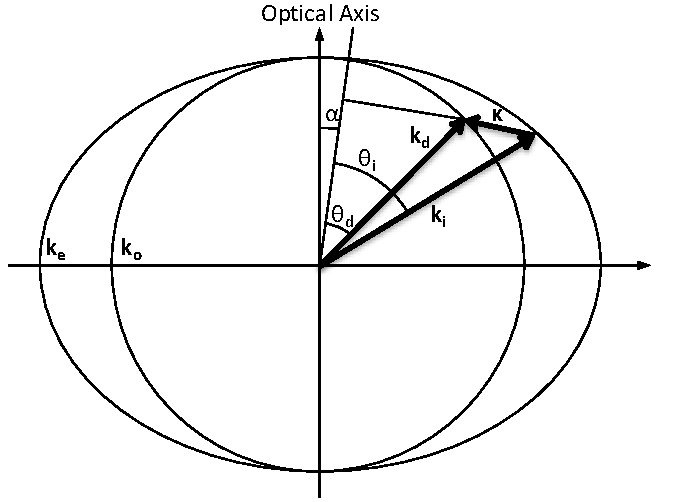
\includegraphics[width=0.7\textwidth]{./Images/3-1-AOTFWavevectorWithRefraction.pdf}
    \caption{The wave vectors generated by the AOTF experiment. From \autoref{eqn:3.1:phaseMatching}, the incident wave vector, diffracted wave vector, and acoustic wave vector are shown.}
    \label{fig:3.1:ATOFWavevectors}
    \end{center}
\end{figure}

\newpage

\begin{figure}
    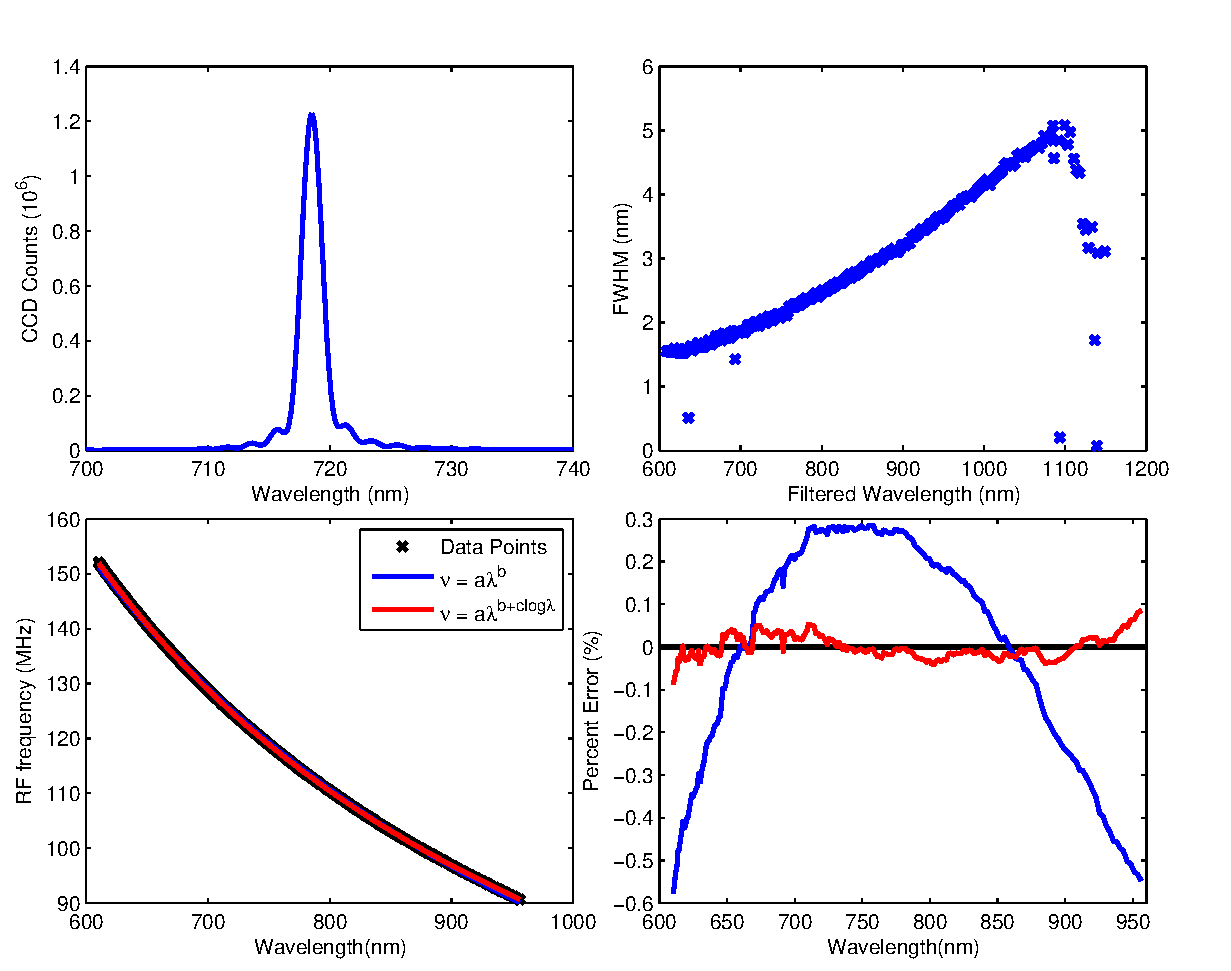
\includegraphics[width=1.0\textwidth]{./Images/3-1-AOTFCharaterization.pdf}
    \caption{(a) A standard image taken from the AOTF calibration experiment when the tuning frequency of the AOTF was at 124.96~MHz. (b) The FWHM for each of the determined wavelengths for the AOTF. The FWHM at 600~nm is 1.5~and as the wavelengths get longer the FWHM increases to 4.9 at 1080~nm. (c) The calibration curves for the AOTF RF versus the  diffracted wavelength which contains the data points recorded and two best fit curves. (d) The percent error with respect to the measured frequency for the two best fit curves in the previous panel.}
    \label{fig:3.1:AOTFCharaterization}
\end{figure}

\newpage

\begin{figure}
    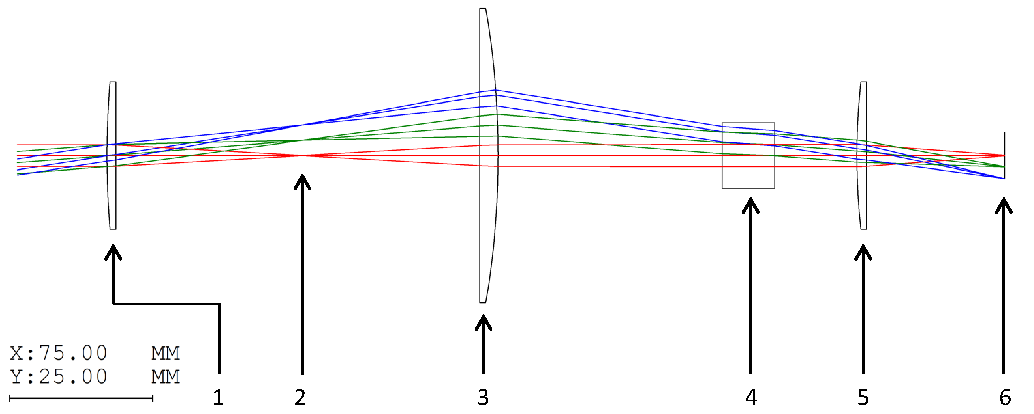
\includegraphics[width=1.0\textwidth]{./Images/3-2-TelescopicRayTracing.pdf}
    \caption{Ray Tracing diagram of the telescopic lens system for ALI simulated by Code V optical design software. The elements in the system are the following: (1) 150~mm focal length plano-convex lens. (2) Slit plate. (3) 100~mm focal length plano-convex lens. (4) Vertical linear polarizer. (5) Brimrose AOTF. (6) Horizontal linear polarizer. (7) 50.4~mm focal length plano-convex lens. (8) Imaging plane.}
    \label{fig:3.2:telescopicRayTracing}
\end{figure}

\newpage

\begin{figure}[h!]
        \centering
        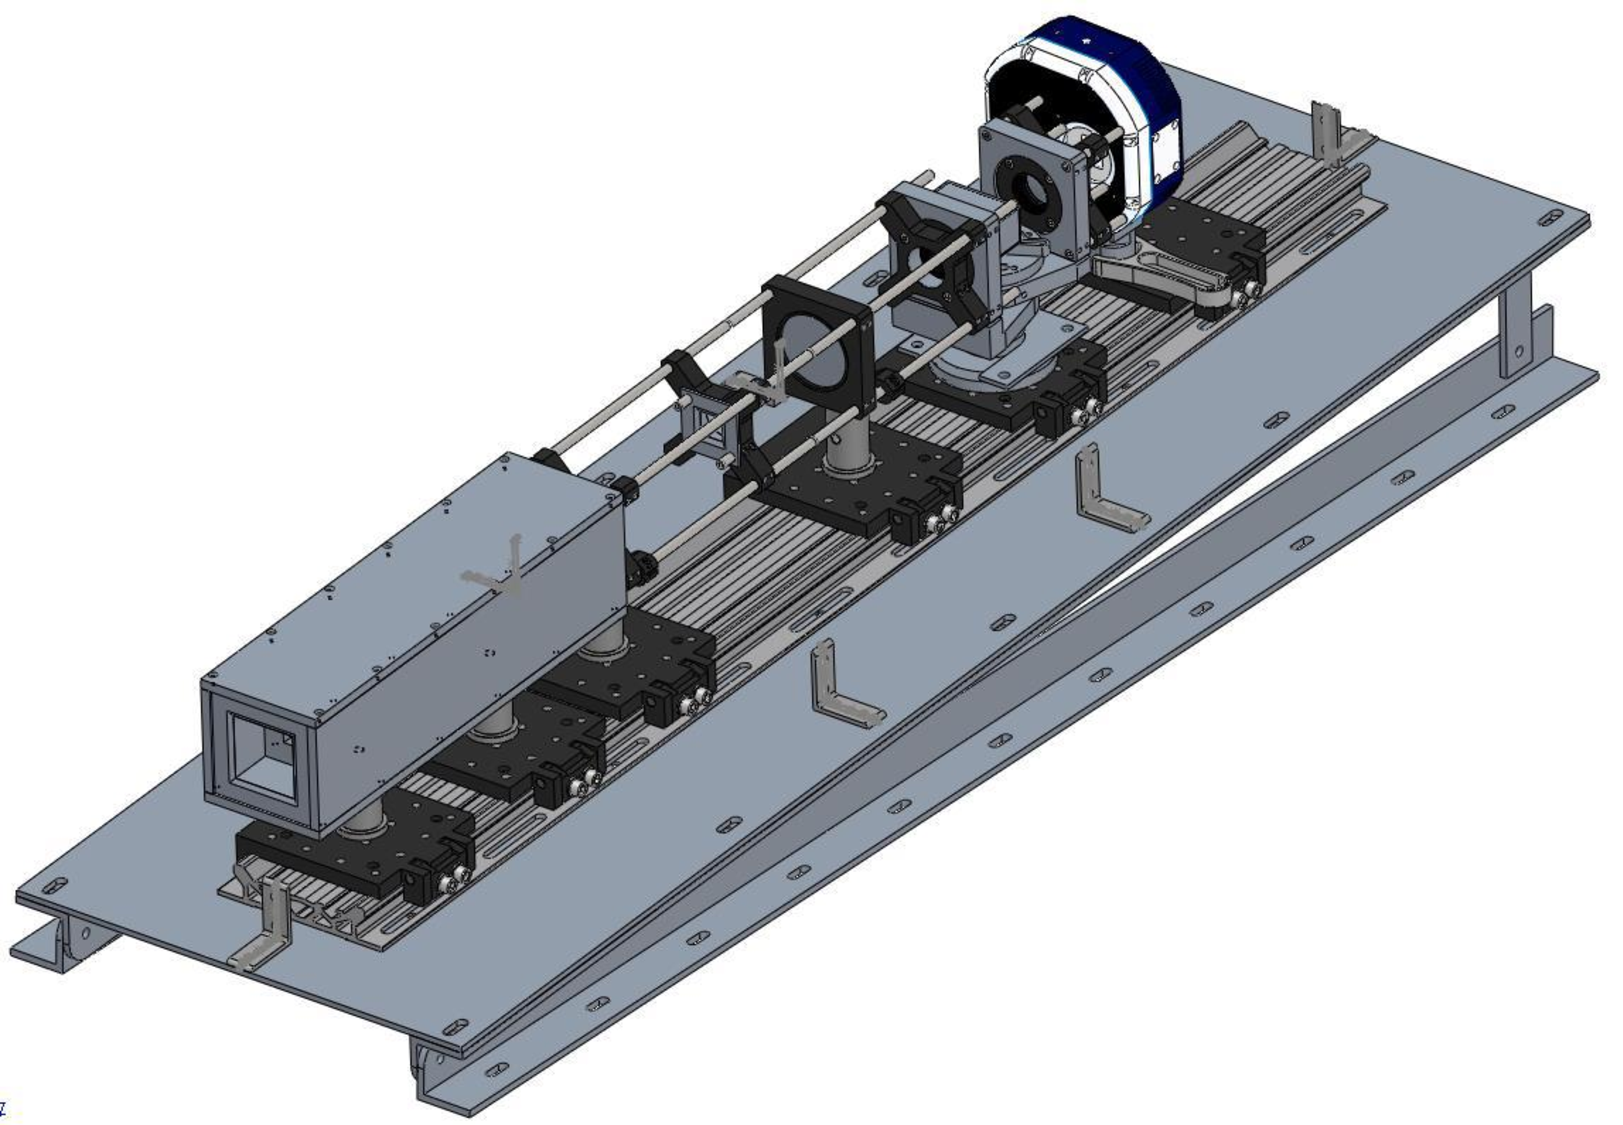
\includegraphics[width=1.0\textwidth]{./Images/3-3-AliCompleteDesign.pdf}
        \caption{An isometric view of the complete ALI system with the baffle and field of view slant. Light tight case absent from diagram.}
        \label{fig:3.3:aliSystemDiagram}
\end{figure}

\newpage

\begin{figure}
    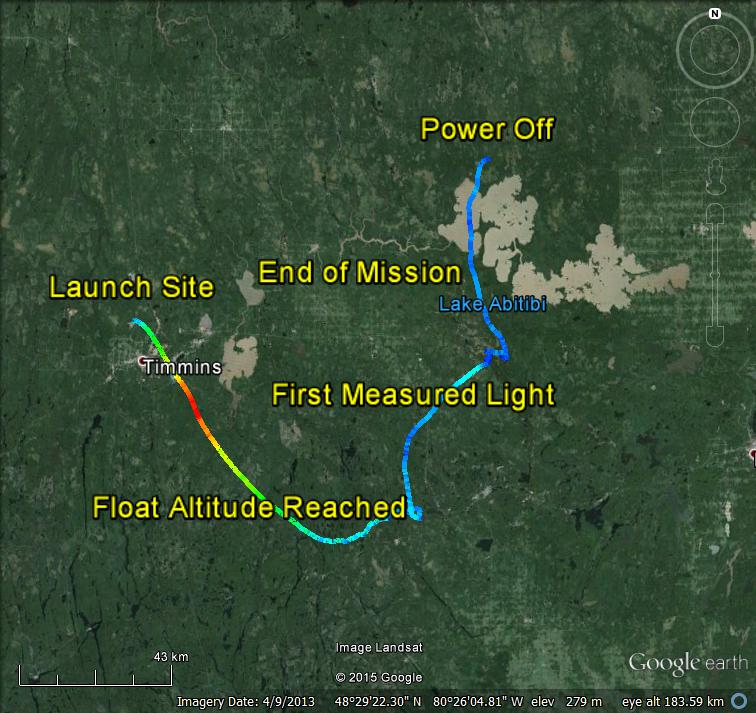
\includegraphics[width=1.0\textwidth]{./Images/5-1-AliGpsDataGoogleMaps.jpg}
    \caption{The GPS data from ALI during the Nimbus 7 mission generated via Google Earth. The colour of the line represents the absolute speed of the gondola during the mission. Important landmarks are noted on the image. The end of mission represent the end of the aerosol mission. No GPS data was collected from ALI after power down.}
    \label{fig:5.1:nimbus7FlightPath}
\end{figure}

\newpage

\begin{figure}
    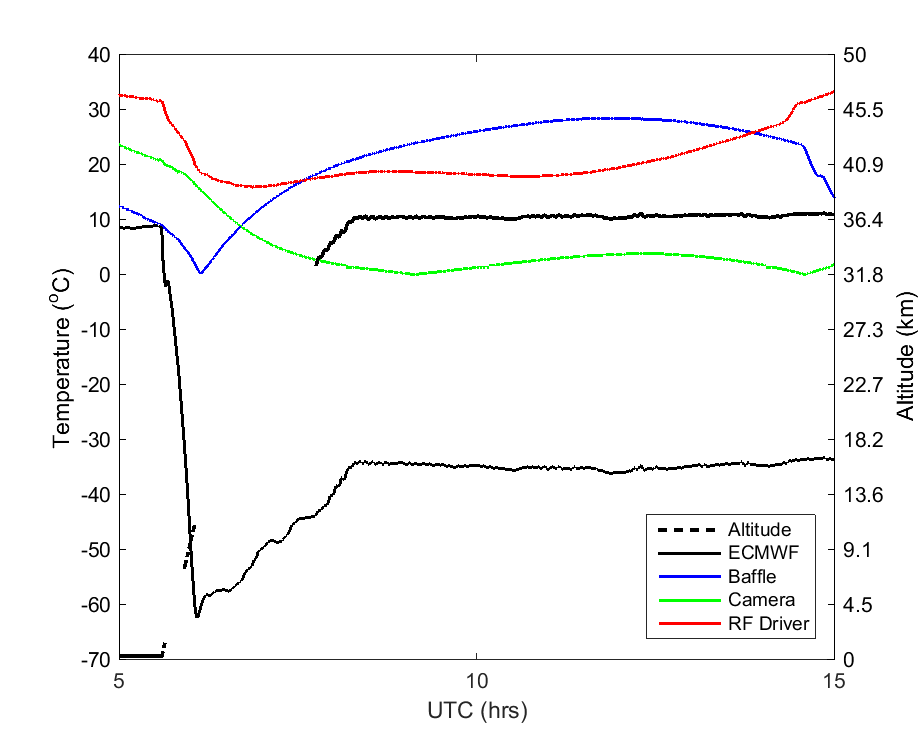
\includegraphics[width=1.0\textwidth]{./Images/5-1-FlightTemperatures.pdf}
    \caption{Temperature and altitude profiles from the NIMBUS 7 flight.}
    \label{fig:nimbus7Temps}
\end{figure}

\newpage

\begin{figure}
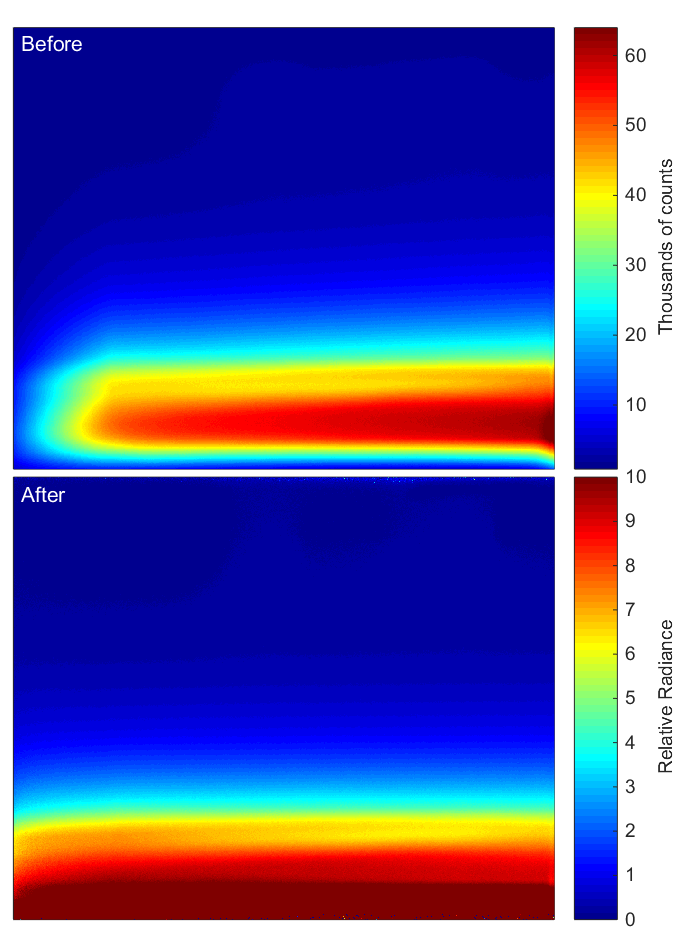
\includegraphics[width=0.5\textwidth]{./Images/5-2-BeforeAfterImage.pdf}
    \caption{Comparison of the same image, image number 212, which is at 750~nm. The upper panel is the raw level 0 data and the lower panel is the relative radiance level 1 data.}
    \label{fig:BeforeAfterImages}
\end{figure}

\newpage

\begin{figure}
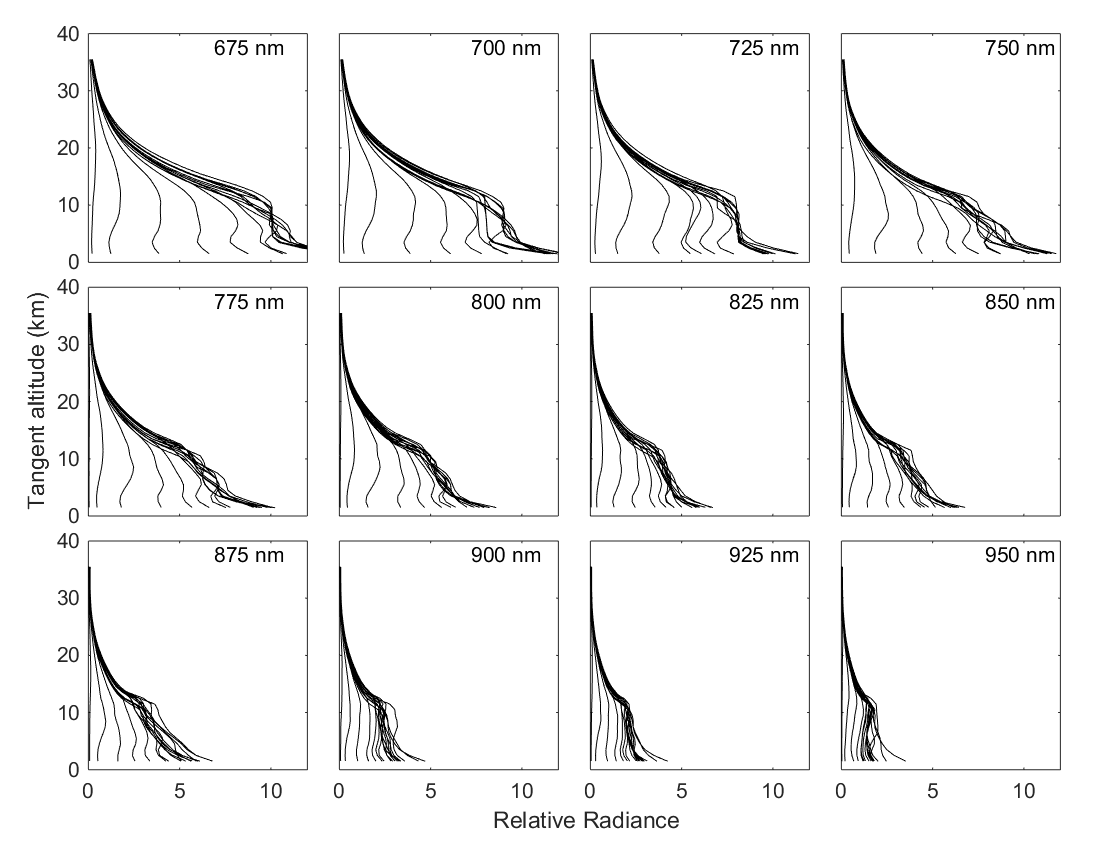
\includegraphics[width=1.0\textwidth]{./Images/5-2-AliRadianceVectors.pdf}
    \caption{All ALI relative radiance vectors from the NIMBUS-7 flight from the straight ahead line of sight averaged to a 1~km resolution. Each panel presents the raidance vectors from a different wavelength measured which is denoted in the top right corner. }
    \label{fig:AliRadiancesVectors}
\end{figure}

\newpage

\begin{figure}
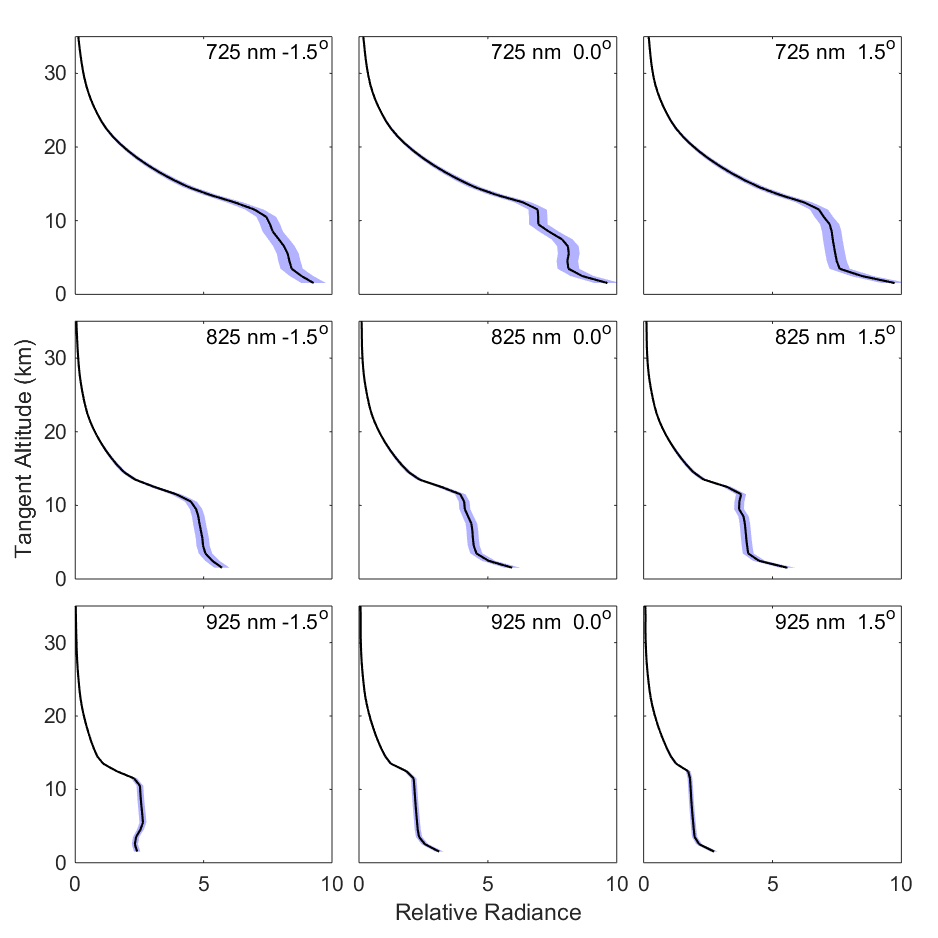
\includegraphics[width=1.0\textwidth]{./Images/5-2-AliRadiancesWithError.pdf}
    \caption{Level 1 relative radiances as measured from ALI at approximately 14:20 UTC (images number 207, 211,and 215) looking 90\si{\degree} from the sun facing southwards. The top middle, and bottom row are measurements taken at 725, 825, and 925~nm respectively. The center column is viewing the atmosphere directly in front of ALI, While the left column is looking to the left at -2.5\si{\degree} and the right at 2.5\si{\degree}. }
    \label{fig:AliRadiances}
\end{figure}

\newpage

\begin{figure}
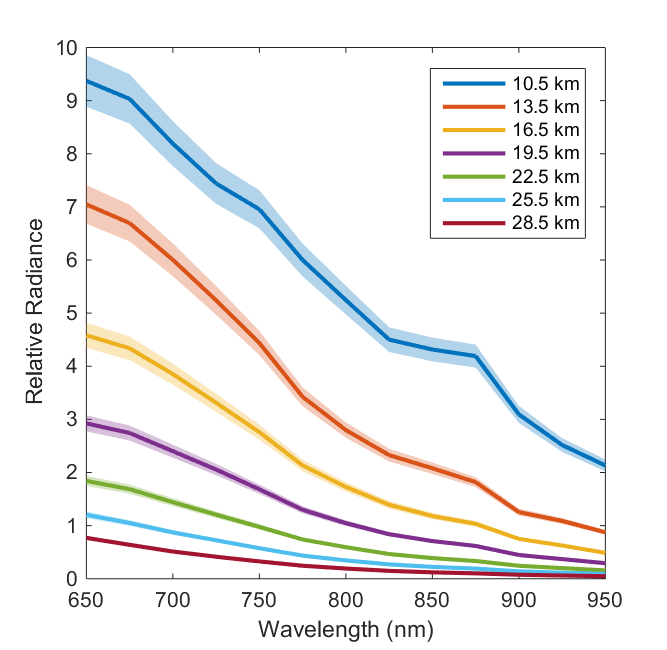
\includegraphics[width=1.0\textwidth]{./Images/5-2-AliSpectralRadiances.pdf}
    \caption{Level 1 relative radiances spectrally from 650~nm to 950~nm as measured from ALI at approximately 14:20 UTC consisting of images number 204 to 216 looking 90\si{\degree} from the sun facing southwards. These spectral profiles are presented at several tangent altitudes with a horizontal look direction of 0\si{\degree}.}
    \label{fig:AliSpectralRadiances}
\end{figure}

\newpage

\begin{figure}
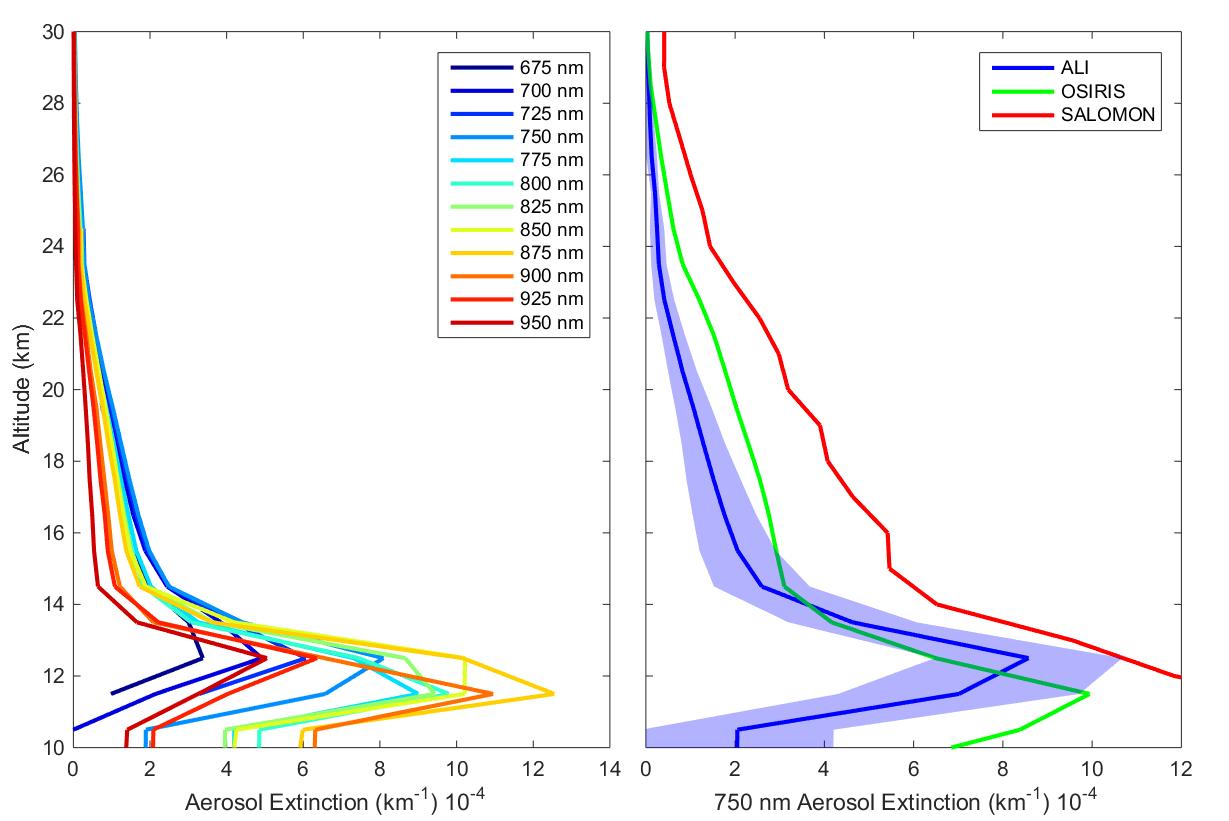
\includegraphics[width=1.0\textwidth]{./Images/5-3-FullAerosolCycleComparison.pdf}
    \caption{Left is the retrieved aerosol extinction profiles from the last complete cycle consisting of images 205 to 216 from the 0.0\si{\degree} horizontal line of sight. Right is the 750~nm ALI aerosol extinction in blue with its error represented by the shading compared to the 750~nm extinction measured by OSIRIS and SALOMON in green and red respectively.}
    \label{fig:AliAerosolCycle}
\end{figure}

%\newpage

%\begin{figure}
%\includegraphics[width=1.0\textwidth]{./Images/5-3-AliRetreivals.pdf}
%    \caption{An example of three aerosol retrievals from images 207, 211, and 215, with center wavelengths of 725, 825, and 925~nm respectively and vertically displayed in the figure from top to bottom. The left column shows the measurement vector, $y$, in black with the retrieved forward model, $F$, in blue. The center column shows the ratio of the $y$ over $F$ known as $\alpha$ and is the convergence factor between the ALI measurement and the forward model. The final column is ALI aerosol extinction in blue with the associated error represented by the light blue shading. The green is 750~nm aerosol extinction measured by OSIRIS, and red is 750~nm extinction as measures by SALOMON.}
%    \label{fig:AliRetreivals}
%\end{figure}

\newpage

\begin{figure}
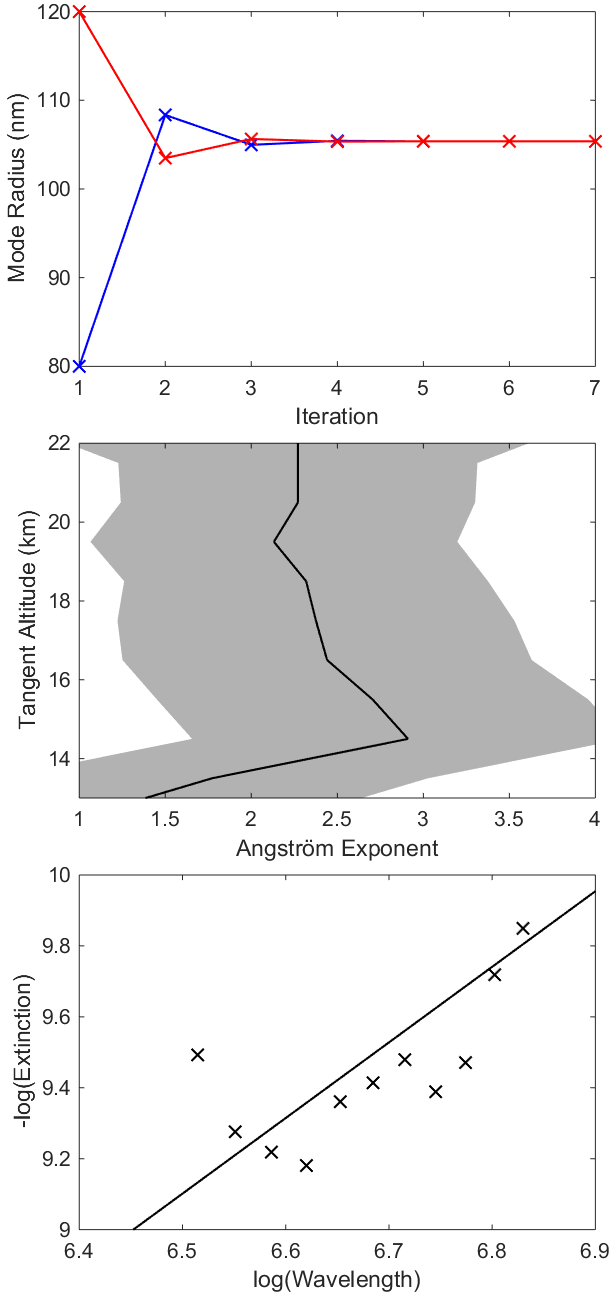
\includegraphics[width=0.5\textwidth]{./Images/5-4-ParticalSize.pdf}
    \caption{The top panel shows the convergence of the mode radius throughout the iterations in the retrieval. The second panel is the final Angstr\"{o}m exponents determined for images 204-217 during the Timmins 2014 campaign. And the last panel demonstrate a least squares fit to determine the Angstr\"{o}m exponent at 20.5~km shell altitude.}
    \label{fig:ParticleSize}
\end{figure}



\end{document} 